\documentclass[a4paper,10pt]{article}
\usepackage{amssymb}
\usepackage{alltt}\tiny
\usepackage{amsmath,amsfonts}
\usepackage{amsthm}
\usepackage{graphicx}
\usepackage{hyperref}
\usepackage{epstopdf}
\DeclareGraphicsExtensions{.pdf,.png,.jpg}
\newtheorem{theorem}{Theorem}[section]
\newtheorem{definition}[theorem]{Definition}
\newtheorem{lemma}[theorem]{Lemma}
\newcommand{\nop}[1]{}

% These are from candidacy edic.tex
\graphicspath{{./graphics/}}
\DeclareGraphicsExtensions{.pdf,.jpeg,.png}

% Legacy from Christoph's paper:
% \DeclareGraphicsRule{.tif}{png}{.png}{`convert #1 `dirname #1`/`basename #1 .tif`.png}

% When converting eps to pdf, suffix is added to filename. 
% Recommended not to be empty string by http://www.tex.ac.uk/tex-archive/macros/latex/contrib/oberdiek/epstopdf.pdf : page 4, suffix paragraph.
\epstopdfsetup{suffix=-generated}

\begin{document}

\title{Milestone 2 Squall/Storm project proposal: Theta joins in Squall}
\date{}
\maketitle

\section{Introduction}
\vspace{2mm}
The goal of this project is to implement a two-way theta-join operator in Squall/Storm, based on the ``Processing Theta-Joins using MapReduce''~\cite{ThetaJoin}, run experiments with the operator and compare it with the traditional approach. Theta-join is a join that takes two relations, and from the cartesian-product matrix built from these relations, specifies a subset which fulfills the join condition and produces the join result. The join condition can be an arbitrarily complex function - i.e. equijoins, inequality joins etc. are all subtypes of theta-join. However, the paper is concerned with traditional, non-online MapReduce systems, so we will have to adapt it in order to use it in the online context. You will implement your code on top of our system, which is described in SquallQuickStart document. There you can also find the definition of term ``online''.

A join consists of a join condition and a join result function. The join condition can either be specified on a cell-by-cell on the join matrix, or as an equijoin, inequality, band or cross-product join. The join result function takes two tuples from a cell as the input and produces (if the join condition is satisfied) a result tuple. Both the join condition and the join result function need to be easily configurable and properly decoupled in the code.

The content of this document is as follows. Subsection~\ref{Foundations} discusses the Theta-Join paper in more details (you will still have to read the original paper). Then, hints about the modifications in the current system, which are necessary for implementing new operator, are given. Third section enumerates experiments you have to run, and the content of the zip archive you have to deliver. The last section presents extra requirements (running directly from SQL) for which you might gain extra points.

\subsection{Theoretical foundations}
~\label{Foundations}
Traditionally, the basic idea for equijoins in MapReduce is that the tuples from both relations with the same join key are sent to the same Reducer, and then inside each Reducer a variant of merge-join is employed. As explained in the paper, there are two downsides of this approach. First, the number of different join conditions limits scalability. For example, in the following query:
\begin{verbatim}
SELECT R.A * S.C FROM R, S WHERE R.B=S.B
\end{verbatim}
with the following schema:
\begin{verbatim}
R(A,B), S(B,C)
\end{verbatim}
assume that R and S have only 3 different values for \verb|B|. That means that we cannot use more than 3 Reducers, no matter how huge \verb|R| and \verb|S| are. Second, there might be a skew in the number of tuples for the distinct values of \verb|B|, and the completion time is determined by the Reducer with the most work.

\textbf{Cross-product joins.} The authors presented a join algorithm which has a different policy for assigning work to Reducers. Namely, each cell (which produces a join result) is assigned to exactly one Reducer. A cell is defined by a row (representing a set of tuples from one relation) and a column (representing a set of tuples from the other relation). A Mapper is responsible for sending a tuple to each Reducer that has an intersection with the row (column) that the tuple belongs to. A Reducer receives tuples from both relations. It has to examine all the pairs of tuples, such that the first tuple belongs to the first relation, and the second tuple belongs to the second relation. For each pair, if the join condition is satisfied, the Reducer produces a join result tuple. A cell for which the join condition is satisfied is denoted as a \textit{candidate cell}.

The paper's main contribution is the observation that careful grouping cells into \textit{regions}, such that each region is assigned to a Reducer, provides near-optimal solutions for cross-product joins. Optimality in this context refers to minimizing both the maximum number of tuples a Reducer receives and the maximum number of tuples a Reducer sends. The former is denoted as \verb#Max-Reducer-Input#, and the latter as \verb#Max-Reducer-Output#. If these regions are actually squares, then we can achieve optimal solutions for both \verb#Max-Reducer-Input# and \verb#Max-Reducer-Output#. Intuitively, a square is a rectangle which covers the largest space with the smallest sum of two sides - in our case, each side is a part of a relation that the region is responsible for. This makes the solution \verb#Max-Reducer-Input#-optimal. Since the squares are of equal size and we have cross-product as the join type, the work each Reducer has to do is also equal. This makes the solution \verb#Max-Reducer-Output#-optimal. See Lemmas 1 and 2 from the paper for a rigorous proof of these claims.

The reason why we are not using multiple small regions per Reducer is presented in Figure 4 in the middle from the paper. We want to avoid sending a tuple (in this case with \verb#S.A=7#) to many Reducers (in this case to three Reducers), because it will unnecessarily increase network traffic. In addition, in the same figure, a \textit{duplicate output} situation might occur. That is, the same pair of tuples is sent to two reducers (in this case \verb|S2| and \verb|T2|) but they will provide the join result for different cells. To mitigate this problem, Mappers need to pass information to a Reducer about the join matrix tuples the Reducer is responsible for.

In order to implement this algorithm (the authors call it 1-Bucket-Theta), we need to know the cardinality of all the relations we want to join. The ideal region will be a square with area $\frac{|S||T|}{r}$, where \verb#|S|# and \verb#|T|# are the relation sizes and \verb|r| is the number of Reducers. Thus, the optimal side length is $a = \sqrt{\frac{|S||T|}{r}}$, and this number is often not an integer. Your task is to create a mapping from a join matrix to Reducers, such that
\begin{enumerate}
 \item each cell belongs to exactly one Reducer,
 \item each region is a square with $a = \sqrt{\frac{|S||T|}{r}}$,
 \item if this is not possible, each region is a square with the side close to optimal,
 \item if this is not possible, each region is a square-like rectangle with the sides close to optimal.
\end{enumerate}

Close to optimal means that no region side is two times or more bigger than the optimal side length. Each region should be of the same size, except a few of those which are close to the borders of a join matrix. A more formal explanation of how to build these regions can be found in Theorem 2 and 3. For example, assume \verb#|S| = 10.000#, \verb#|T| = 30.000# and \verb#r = 5#. $\frac{|T|}{r} < |S|$ fulfills the condition of Theorem 3, and the optimal square side would be \verb#a $\approx$ 7746#. However, the closest to optimal are regions such that the join matrix is partitioned in a single row of 5 rectangles, each of \verb#|S|*|T| = 10.000 * 6.000#. In the \verb#|S|# dimension, the side is \verb#1.29 * optimal_side_legth#. In the \verb#|T|# dimension the side is \verb#0.77 * optimal_side_length#. For a given \verb|a|, theoretically \verb#Max-Reducer-Input =  7746 + 7746 = 15.492# would be the best. However, in this particular example, we cannot achieve this. Actually, our solution has \verb#Max-Reducer-Input =  16.000#, so it is very close to the theoretically optimal solution. Indeed, it is the best one for this example, being optimal for \verb#Max-Output-Reducer#, and only 3.2\% worse than the theoretically optimal \verb#Max-Input-Reducer#. You can try different regions to see other solutions.

Interestingly, the paper didn't anticipate side lengths less than optimal in Theorem 3. In Theorem 2, the authors showed that single row blocking is the optimum, but for different conditions.

To conclude, by having regions of equal size, we achieve the optimal \\ 
\verb#Max-Reducer-Output#, since each Reducer has exactly the same number of join result tuples to produce. In terms of \verb#Max-Reducer-Input#, we are as close to the optimal solution as the regions are more square-like (side lengths differ slightly).

\textbf{The necessity for randomization.} In a parallel system, it is hard to assign each tuple a unique serial number. The authors opted not to use a consensus algorithm. Instead, they resorted to a simple trick. Each tuple is assigned a random number from the range \verb#[1, cardinality]# where \verb#cardinality# is the total number of tuples that will be emitted from the relation that the tuple belongs to. As a side effect, we get one more benefit: load-balance of Reducer outputs in the presence of an arbitrary theta-join. For example, some regions might produce no join tuples, whereas others might produce many. By shuffling rows/columns of the join matrix, a skew is avoided. Thus, it is essential to have a good randomization function, which scatters tuples uniformly.

\textbf{Sparse join matrices: discarding whole regions.} 
Now, we will distinguish query types by the percent of candidate cells within a join matrix. We denote this percent as \textit{selectivity}. \textit{Input-dominated} query is a query in which the total number of tuples from the two joined relations is bigger than the number of join result tuples. In the example from the paper, the percentage was 0.0000003\%. \textit{Output-dominated} query is a query in which the total number of tuples from the two joined relations is orders of magnitude smaller than the number of join result tuples. In their example, the percentage was 0.088\%.

Thanks to randomization, it is practically impossible to beat the\\
\verb#Max-Reducer-Output# optimality of 1-Bucket-Theta algorithm. However, Mappers might send tuples to Reducers which produce no join result tuples. The authors showed in Section 4.2 that the cost cannot be degraded more than a $\frac{2}{\sqrt{x}}$, where \verb#x# is the selectivity of the query. For example, for \verb#x = 50%#, the cost is at most 3 times bigger than the optimal one. This is the worst-case which we might encounter when the join matrix is a row (or a column) of regions. If we have a grid of regions, with at least 2 regions per column and row, we have a guarantee that the cost is at most 2.12 times bigger than the optimal one. (For more information, please consult Section 4.2 of the paper). 

If a region contains no candidate cells, it can safely be discarded, without being assigned to any Reducer. For example, in an inequality join in which about 50\% of cells do not contribute to the final result, so that many regions can be discarded. The phenomenon that a tuple is sent to many more Reducer than necessary is denoted as \textit{tuple duplication}. However, in an online system we have no guarantees over the order tuple arrivals, and we don't want to block until tuples are sorted. Thus, it makes it practically impossible to find relatively large areas with no candidate cells. The randomization further complicates things. In order to discard some regions, randomization must be turned off and an additional MapReduce phase for collecting statistics has to be employed, which is not feasible in online systems. So we refrain from using M-Bucket-I and M-Bucket-O, and use only 1-Bucket-Theta algorithm.

To conclude: assigning regions with no candidate cells to Reducers certainly leads to a slowdown in Input-dominant queries. To mitigate this problem, an additional MapReduce phase for collecting statistics is required, which is not feasible in an online system. Nevertheless, in most cases we are interested in Output-dominated queries.

\textbf{Equijoin insight.} Although the authors of the paper claim their algorithm can be used to avoid skew in equijoins, we will see that this does not completely hold. When performing an equijoin using the cross-product technique, as shown in Figure 5 from the paper, \verb#Max-Reducer-Input# is 8 and \verb#Max-Reducer-Output# is 4, which is exactly the same as in the random matrix-to-reducer mappings from Figure 4 from the paper. This emphasizes once more that tuple duplication is the main problem of the theta-join algorithm. However, the theta-join algorithm attains a better \verb#Max-Reducer-Output# value.

To conclude: the traditional equijoin implementation achieves better performance than the corresponding implementation using the theta-join algorithm when:
\begin{enumerate}
 \item the query is input-dominated, and 
 \item data is not skewed much.
\end{enumerate}

\subsection{Theta-join inside Squall/Storm}
The previous subsection promoted using theta-joins. However, the take-away point was the algorithm for efficiently constructing regions from a join matrix.

The global architecture of a Theta-join component is presented in Figure~\ref{fig:ThetaJoinComponent}. Input stream from a previous component is uniformly partitioned across a layer of nodes that we call the \textit{Shuffle layer}, independently of a tuple's join condition key. The Shuffle layer is responsible for sending a tuple to a ResultProducer node(s). The Shuffle and ResultProducer layers work analogously to Map and Reduce phases. The \verb#r# constant from the paper refers to the number of nodes in ResultProducer level here. Keep in mind that you are responsible for specifying a connection not only between Shuffle and ResultProducer layers, but also between the previous query component and the Shuffle layer, as well as between the ResultProducer layer and the next query component. For more information about interconnecting components, please refer to the \verb#Stream groupings# section of \url{https://github.com/nathanmarz/storm/wiki/Concepts}. You might also need \verb#CustomStreamGrouping#, so please consult \url{http://nathanmarz.github.com/storm/doc-0.7.0/index.html}. You will need to make necessary changes in the \verb#components# and \verb#stormComponents# package. The former defines a user interface for a component (this is where you define the type and parameters of a query). The latter specifies a bridge between Squall and Storm. Namely, it translates user-defined join characteristics into Storm-understandable settings.

\begin{figure}
\centering
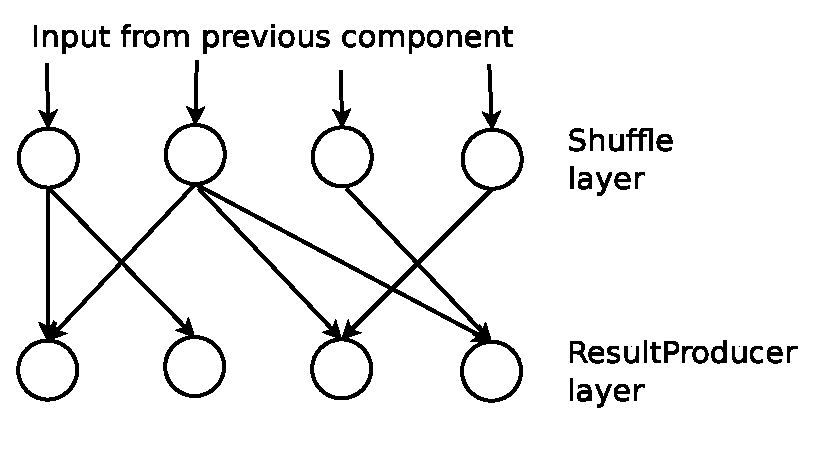
\includegraphics[width=3in]{ThetaJoinComponent.eps}
\vspace{-3mm}
\caption{ThetaJoinComponent layers: the arrow(s) between a Shuffle node and a ResultProducer node(s) represents a possible shuffling for a single tuple.}
\label{fig:ThetaJoinComponent}
\vspace{-2mm}
\end{figure}

Inside each ResultProducer node, an arbitrary join strategy can be used. You can adopt the strategy from JoinComponent. When a new tuple arrives, you can perform a join with the full content of the opposite relation. You can apply an optimization which allows you to not scan over the whole opposite relation. However, keep in mind that this optimization is not generic, rather it depends on the query. A user of your class is not supposed to change the code inside, but only to instantiate the class with the appropriate parameters.

\textbf{Scalability.} The authors argued that higher \verb#r# we use, the less skew we might have (Section 4.1.1). Our cluster has 176 nodes, out of which 17 are Ackers, and some of them are also dedicated to other operators in the query plan. Keep in mind that the network traffic might cause your operator to not scale after some \verb#r#. You have to report this threshold value and show it on graphs. In addition, our online processing system is a main-memory system, so keep in mind that the maximum heap size for Squall Java processes is constrained (on cluster it is around 1GB). When the memory used is close to this amount, the system slows down drastically, and when it reaches the bound it does not report an \verb|OutOfMemoryException|, but rather the topology fails some tuples, so that you have to kill your topology. Memory aware solutions are not feasible in the online context, since some tuples need to be batched. 

\textbf{An optimization.} You might also merge the Shuffle layer with the previous component, but keep in mind that in that case you have to modify all the other existing components. Also, in the future, we might add more of them, so if you decide to implement this optimization, make sure it is robust enough.

%avoid duplicate output -the problem increases with the number of reducers.
%You are not obliged to implement Memory Aware version, but if you decide to do so, a way to avoid duplicate output must also be implemented.

\subsection{Experiments}
You will experiment with TPCH queries and DBGEN-erated databases. You can do all the experiments by slightly modifying the \verb#HyracksPlan#. By specifying different join condition, you can make the query Input- or Output-dominant. You will also have to use skew data, and now we will explain how you can generate it.

\subsubsection{Generating skew data}
In order to perform experiments with skewed data, we provide you a modified TPCH databases where the columns have non-uniform (skewed) data distributions. These datasets are generated using a modified version of DBGen program which can be found in \verb#INSTALL_DIR/install/auxiliary/tpch_skew#. The program is capable of generating data from a Zipfian distribution, where the Zipf value (z), which controls the degree of skew in the data, is a parameter that can be specified to the program. For example, the parameter z=0 generates a uniform distribution for each column in the database, whereas z=4 generates a highly-skewed distribution (i.e., a few values occur very frequently) for each column. 

\textbf{Compilation.} The modified DBGEN is pre-compiled for Mac and Solaris. If you want to compile it for Linux, you have to run the following:
\begin{verbatim}
cd $INSTALL_DIR/install/auxiliary/tpch_skew
cp makefile_linux makefile_linux
make clean
make
\end{verbatim}

If you want, you can also recompile it for other operating systems, by using \verb#makefile_MacSolaris#:
\begin{verbatim}
cd $INSTALL_DIR/install/auxiliary/tpch_skew
cp makefile_MacSolaris makefile
make clean
make
\end{verbatim}

\textbf{Running.} You will need to create a skew database for Local Mode and refer to it properly from your config files. In Cluster Mode, you can use a set of predefined databases available at \verb#/export/home/avitorovic/queries/skew_tpch#. We generated datasets with different skew values (1,2,3,4) for scaling factors 1 and 10.

The following commands generates a TPC-H database with the scaling factor 1 where data in each column is created from a Zipfian distribution where the degree of skew is 2:
\begin{verbatim}
cd $INSTALL_DIR/install/auxiliary/tpch_skew
./dbgen -s 1 -z 2
\end{verbatim}

\subsubsection{Deliverable}
The result graphs should clearly present:
\begin{enumerate}
 \item The performance difference between the traditional equijoin implementation (available in the \verb#JoinComponent#) and the theta-join implementation of equijoin, both with and without skew
 \item The performance difference between Input- and Output-dominant inequality joins.
 \item The final result for each query you were running - to make sure the results are correct, you can compare with a traditional database, such as MySQL.
\end{enumerate}

You should submit:
\begin{enumerate}
 \item Detailed documentation of the code with the required graphs. If you had to change some of the existing classes, you have to explain exactly what you changed and why it was necessary.
 \item Source code. Separate changed from new classes.
\end{enumerate}

These are set of mandatory SQL queries you need to experiment with (you can write more if you want):
\begin{verbatim}
 1. Hyracks (you already have query plan for this query)
 2. An example of Input-dominated query 
    (around 134000 tuples our of 600.000x150.000 matrix):
    SELECT SUM(LINEITEM.EXTENDEDPRICE*(1-LINEITEM.DISCOUNT))
    FROM LINEITEM, ORDERS
    WHERE LINEITEM.ORDERKEY = ORDERS.ORDERKEY AND 
          ORDERS.TOTALPRICE > 10*LINEITEM.EXTENDEDPRICE
 3. An example of Output-dominated query is a cross product:
    SELECT SUM(SUPPLIER.SUPPKEY)
    FROM SUPPLIER, NATION
 4. An example of a query containing multiple join operators:
    SELECT SUM(LINEITEM.EXTENDEDPRICE*(1-LINEITEM.DISCOUNT))
    FROM LINEITEM, ORDERS, NATION, SUPPLIER, PARTSUPP
    WHERE LINEITEM.ORDERKEY = ORDERS.ORDERKEY AND 
          ORDERS.TOTALPRICE > 10*LINEITEM.EXTENDEDPRICE AND
          SUPPLIER.SUPPKEY = PARTSUPP.SUPPKEY AND
          PARTSUPP.PARTKEY = LINEITEM.PARTKEY AND 
          PARTSUPP.SUPPKEY = LINEITEM.SUPPKEY AND
          PARTSUPP.AVAILQTY > 9990

\end{verbatim}
In \verb#INSTALL_DIR/dip/Squall/src/queryPlans# you can find examples of query plans. Beside Hyracks, we implemented TPCH3, 4, 5, 7 and 8.

%\textbg{Bonus.} This will bring you extra points. The goal is to implement a grid-based theta-join, \verb#GridJoinComponent#. This implementation avoids \textit{input duplication}. Input duplication occurs when a tuple is sent to many reducers, out of many will not use it for producing a result tuple. Avoiding input duplication becomes extremely important where join condition is fulfilled for small portion of join matrix (less than 50\%), that is when a join is input-dominated. 

%\verb#GridJoinComponent# has two layers as in \verb#ThetaJoinComponent#, but ResultProducer tuples. That is, all the tuples with the same join It is not skew-resistant.

\section{Theta join operator and SQLplugin}
\label{ch:Appendix}
\vspace{2mm}

You can earn extra points by implementing the ThetaJoinOperator straight from SQL, by using a plugin for Squall, called SQLPlugin. You can find more information in SquallQuickStart document.

{
\bibliographystyle{ieeetr}
\bibliography{refs}
}

\end{document}